\chapter{Komponentensemantik}
ST: Komponenten-Realisierungssemantik: Komponenten-Diagramm mit
interner Klassenstruktur;
Komponenten-Benutztsemantik: Komponenten-Diagramm mit expliziten
Schnittstellen ohne interne Klassenstruktur;

\subsubsection*{Komponentendiagramm}
... bieten eine standardisierte Möglichkeit um die zuvor genannten Nutzer und ihre Use Cases sowie die Beziehungen zwischen Use Cases untereinander darzustellen.

\textbf{externe Sicht}
\begin{figure}[hbt]
  \centering
  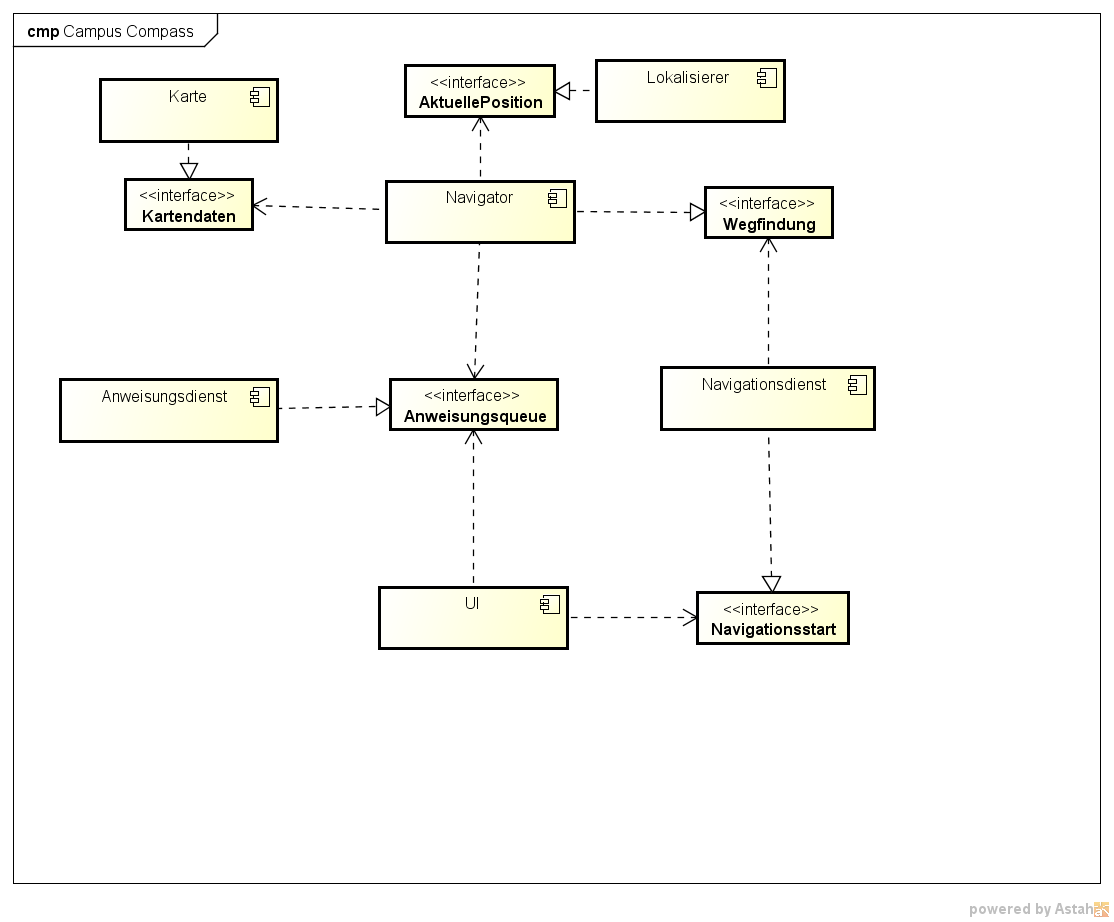
\includegraphics[width=\linewidth]{img/komponentendiagramm.png}
  \label{img:komponentendiagramm}
  \caption{Komponentendiagramm}
\end{figure}

\textbf{interne Sicht}
siehe Klassendiagramm...